\section{3.态叠加原理}

\begin{frame}
    \frametitle{前情回顾}
    \begin{itemize}
        \Item 波粒二象性
        \Item 波函数假说
        \Item 波函数统计诠释
    \end{itemize}
\end{frame}  

\subsection{态叠加原理实验基础}

\begin{frame}
    \frametitle{两种实验}
        \begin{figure}
            \centering
            \subfigure[小球双缝实验]{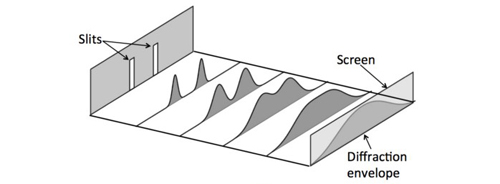
\includegraphics[width=0.495\textwidth]{figs/2022-01-17-13-50-38.png}}
            \subfigure[电子双缝实验]{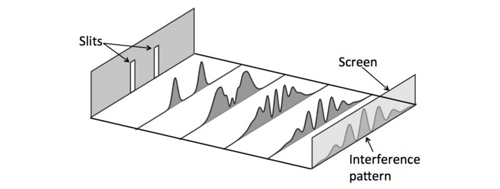
\includegraphics[width=0.495\textwidth]{figs/2022-01-17-13-51-15.png}}
        \end{figure}
    \setcounter{subfigure}{0}
\end{frame}

\begin{frame}
    \frametitle{小球双缝实验}
    \begin{center}
        \includegraphics[width=0.5\textwidth]{figs/sup-2.png} \\
    \end{center} 
    依据统计解释,振幅是概率幅\\
    \begin{itemize}
        \Item 小球双缝实验,$P'=P_1+P_2 $, 是概率叠加。
        \Item 结论:经典叠加服从概率叠加
    \end{itemize}
\end{frame} 


\begin{frame}
    \frametitle{电子双缝实验}
    \begin{center}
        \includegraphics[width=0.5\textwidth]{figs/sup-3.png} \\
    \end{center} 
    依据统计解释,振幅是概率幅\\
    \begin{itemize}
        \Item 电子双缝实验,$P\neq P_1+P_2 $,量子叠加服从的不是概率叠加!
        \Item 波恩认为服从波函数(态)叠加,即:
        $$ \psi =\psi_1+\psi_2$$
    \end{itemize}
\end{frame} 


\begin{frame} [allowframebreaks=]
    Analysing the two-slit experiment:\\
    \begin{itemize}
        \Item Using wavefunction $\psi_1$ to describe the state of the electron running across slit-1 and $\psi_2$ for slit-2. \\
        \Item when the both slits opened, one can assume that the electron locates at the superposition state
            \[ \Psi=c_1 \psi_1+ c_2\psi_2 \]
        \Item based on statistical interpretation, the possiblity density of electron reaches certain point of screen should be
        \begin{equation*}
        \begin{split}
            \omega &=|\Psi|^2 \\
            &= (c_1 \psi_1+ c_2\psi_2)^* (c_1 \psi_1+ c_2\psi_2) \\
            &=(\psi_1^*+\psi_2^*)(\psi_1+\psi_2) \\ 
            & = |c_1|^2 |\psi_1|^2 + |c_2|^2 |\psi_2|^2  + [c_1 c_2 ^* \psi_1 \psi_2 ^* + c_1 ^* c_2 \psi_1 ^* \psi_2] \\
        \end{split} 
        \end{equation*}
        \Item Thus, the interference pattern comes from the item  
        \[[c_1 C_c ^* \psi_1 \psi_2 ^* + c_1 ^* c_2 \psi_1 ^* \psi_2] \]
    \end{itemize}
    \begin{itemize}
        \Item 概率计算表明,电子处于叠加态时,存在干涉项(后两项),产生干涉条纹
        \Item 如果电子不处于叠加态,即电子只过一个缝,则有$\psi_1$ 或$\psi_2$为零,不存在干涉项为,没有干涉条纹!
        \Item 干涉条纹正是源于电子同时过两个缝的状态, 即叠加态。
    \end{itemize}
    基于此,波恩提出了态叠加原理
\end{frame}

\subsection{态叠加原理表述}

\begin{frame}
    \frametitle{态叠加原理}
    Born also proposed that: \\
    \begin{tcolorbox4}[Superposition principle of states]
    If $\psi_1$ and $\psi_2$ are the possible states of the system,
    their linear superposition \[ \Psi=c_1 \psi_1+ c_2\psi_2 \]
    is also the possible state of the system.\\
    if the system locates at the superposition $\Psi$, the possiblity of observating the system at $\psi_1$ is $|c_1|^2$, and at $\psi_2$ is $|c_2|^2$ \\
    \[|c_1 |^2 + |c_2 |^2 =1\]
    \end{tcolorbox4}
\end{frame}

\begin{frame}
    \frametitle{}
    \begin{tcolorbox4}[态叠加原理中文表述]
    如果 $\psi_1$ 、 $\psi_2$、 $\cdots$、$\psi_N$ 是粒子可能的态,那么它们的线性叠加
        $$ \Psi=c_1 \psi_1+ c_2\psi_2+\cdots+c_N\psi_N $$
    也是粒子可能的态(叠加态)\\   
    如果粒子处于叠加态 $\Psi=\sum\limits_{i=1}^N c_i \psi_i$,  
    那么测得粒子处在第$i$态 ($\psi_i$) 的概率为 $|c_i |^2$, 
    并且有  $$\sum_{i=1}^{N} |c_i|^2 =1$$
    \end{tcolorbox4}
\end{frame}

\subsection{波函数坍塌}

\begin{frame}
    \frametitle{实验升级}
    \begin{center}
        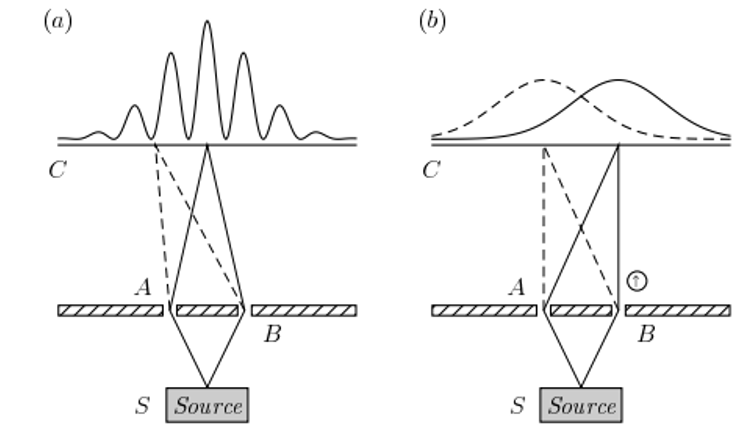
\includegraphics[width=0.5\textwidth]{figs/sup-4.png} \\
    \end{center} 
    \begin{itemize}
        \Item 目标:想观测到电子是如何同时过两个缝的
        \Item 结果:1)只能测到电子要么过第一缝,要么过第二缝。\\
        2)探测器越灵敏,干涉条纹越模糊,\\
        3) 当探测器能长时间地保持几乎可以完全判断电子过哪条缝时,干涉条纹消失!如图(b)所示
    \end{itemize}
\end{frame}

\begin{frame} 
    \frametitle{结果分析}
    \begin{enumerate}
        \Item 实验目标与实验结果的一致性\\
        \begin{itemize}
            \Item 当我们“挖出”A和B两条狭缝时,“设计”了一个想要观察“波动性”的设备,也就是电子已经预先被我们设定为“波”,因此观测到波动性(干涉条纹)
            \Item 当我们装上侦测器时,整个实验被我们“设计”成观察“粒子性”,因为想要知道电子到底是由A还是B穿过,就必须先具备确定的“位置”,因此观察到粒子性(干涉条纹消失)
        \end{itemize}
        \Item 测量可导致状态改变与实验结果的一致性 \\
        \begin{itemize}
            \Item 探测前,电子处于叠加态($ \psi =\psi_1+\psi_2$)
            \Item 探测时,电子状态改变,被迫从叠加态变为确定态 ($\psi_1$ or $\psi_2$),(称为波函数坍塌)
            \Item 探测后,电子处于某确定态,不能干涉。
            \Item 探测器不灵敏,有部分没有被探测到的电子处于叠加态, 干涉条纹模糊。
            \Item 探测器灵敏,全部电子被探测,没有电子处于叠加态, 干涉条纹消失。
        \end{itemize}
        ~~\\
        \Item 测量结果的互补性(互补性原理)\\
        \begin{itemize}
            \Item 波动性和粒子性是两种不同的属性,一般不能用同一设备进行测量
            \Item 不能因为测得粒子性就否定波动性,反之亦然。
            \Item 测量结果就算相互矛盾,也要同时接受,因为它们互补地揭示物体的本质。
        \end{itemize}
        \Item 结论
        \begin{itemize}
            \Item 电子具有波粒二象性,总是处于叠加态
            \Item 不被测量,则保持在叠加态
            \Item 测量导致确定态,但结果是随机的。
            \Item 测得电子某个确定态,不能说明电子原本就处于这个态
        \end{itemize}
    \end{enumerate}
\end{frame}

\begin{frame}
    \frametitle{学术大讨论!}
    The probabilistic interpretation was controversial from the beginning of of quantum mechanics
    \begin{tcolorbox4}[Which Way?]
    \begin{itemize}
        \Item De Broglie : Pilot waves
        \Item Schr$\ddot{o}$dinger: Schr$\ddot{o}$dinger's cat
        \Item Einstein: EPR paradox
        \Item Wheeler's delayed choice experiment
        \Item Quantum eraser experiment
        \Item $\cdots \cdots$
    \end{itemize}
    \end{tcolorbox4}
\end{frame}

\begin{frame}
    \frametitle{薛定谔的猫}
    \begin{center}
        \includegraphics[width=0.8\textwidth]{figs/cat.jpeg} \\
    \end{center} 
\end{frame}

\begin{frame}
    \frametitle{EPR佯谬}
    \begin{center}
        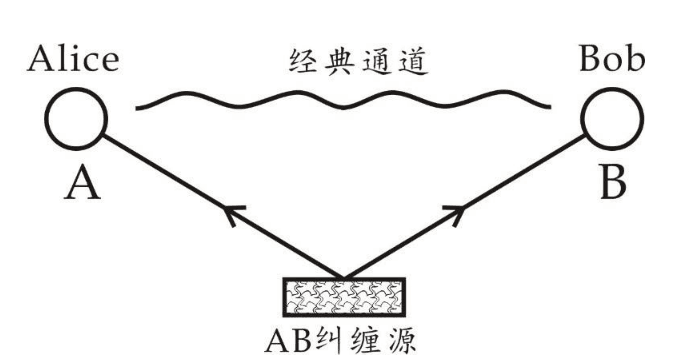
\includegraphics[width=1.0\textwidth]{figs/2022-01-09-14-45-26.png} \\
    \end{center} 
\end{frame}

\begin{frame}
    \frametitle{贝尔不等式}
    \begin{center}
        \includegraphics[width=0.8\textwidth]{figs/bell.png} \\
    \end{center} 
\end{frame}

\begin{frame}
    \frametitle{惠勒延迟选择实验}
    \begin{center}
        \includegraphics[width=0.8\textwidth]{figs/choose.png} \\
    \end{center} 
\end{frame}

\begin{frame}
    \frametitle{量子擦除实验}
    \begin{center}
        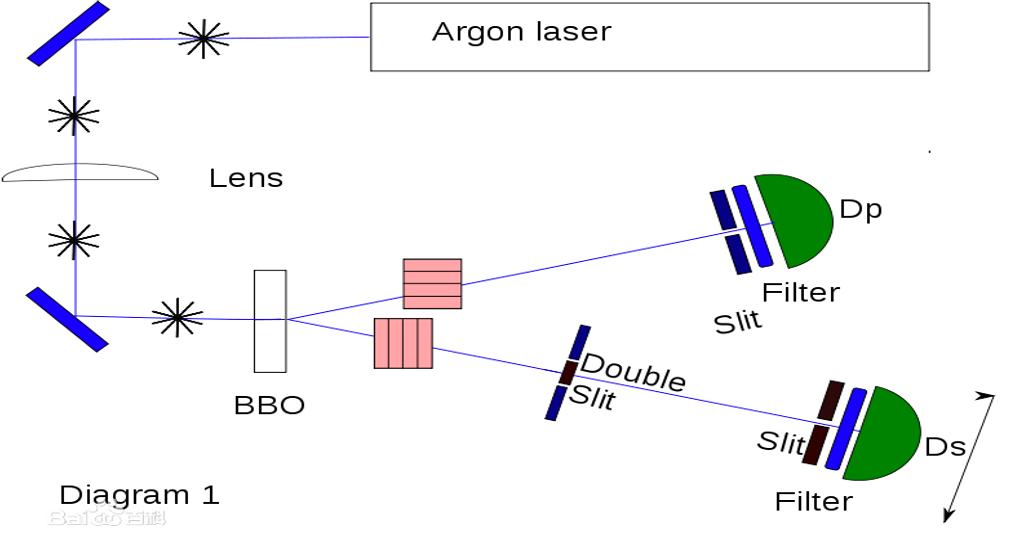
\includegraphics[width=1.0\textwidth]{figs/chachuexp.png} \\
    \end{center} 
\end{frame}

\begin{frame}
    \frametitle{}
    \begin{center}
        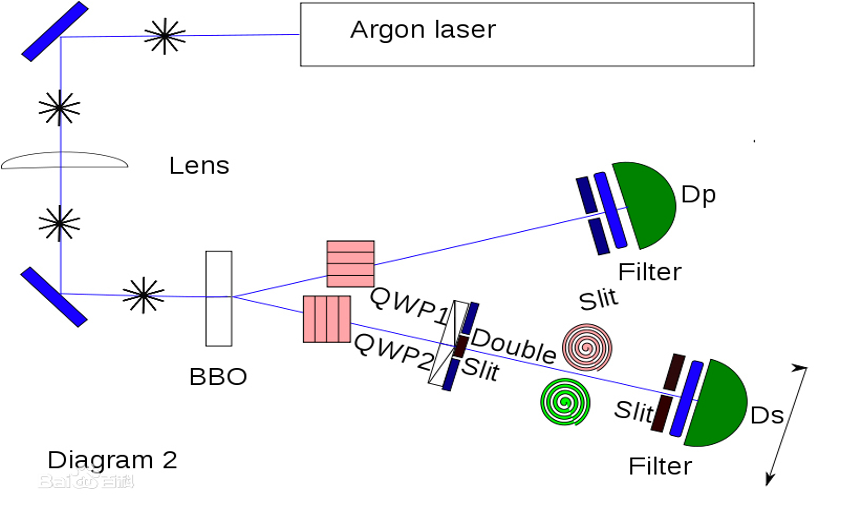
\includegraphics[width=1.0\textwidth]{figs/chachuexp_2.png} \\
    \end{center} 
\end{frame}

\begin{frame}
    \frametitle{}
    \begin{center}
        \includegraphics[width=1.0\textwidth]{figs/chachuexp_3.png} \\
    \end{center} 
\end{frame}

\begin{frame}
    \begin{tcolorbox4}[Conclusion]
        ~~\\
    \begin{enumerate}
        \Item Objects are wave-particles and in superposition state
        \Item Measurement changes the state and gives random results
        \Item Measurement results are complementary
        \Item Measurement leads to objective reality
    \end{enumerate}
    \end{tcolorbox4}
\end{frame}

\begin{frame}
    \frametitle{}
    \centering
    \tcbb[0.5]{Big problems}
    {
      \large  {The world is not a real world?\\
      What is the measurement? \\
      If not performing measurement, what it would be?}
    }
\end{frame}
